% !TeX root = ./pf2020.tex

%\includeonlyframes{current}

\begin{frame}{The language of a computer}
  \begin{itemize}[<+->]
  \item A \textit{computer} is a device that executes programs
  \item A \textit{program} is a collection of instructions to perform a specific
    task
  \item For a computer to understand instructions, these need to be expressed in a
    language that the computer can understand
  \end{itemize}

\end{frame}

\begin{frame}[fragile]{Binary language}

\begin{semiverbatim}
{\color{gray}\tikzref{markbit}0010\tikzref{markbyte}1001110110011000011111010111001011100111101100
11101000101001101011100111111100011101001000011010
00000110001101000011111010010001000101110000010010
00111011010111101101111110110011011111101100101101
10010010110011001101110011000011001011000001010010
11110100101111010001111001011000000000001111110100
1001110101100011010100\tikzref{ins}011100000001\tikzref{ins2}11000011\tikzref{ins3}01001101
00010001111001101000111100100110110110001101100100
01000110010111100011100010100101011011000110010001
10100011111101101000000000111101000001000100101101
11101100011010111001111110010101010110010010000100
00000010010011111010111011011101110011101100000111
00001001111011000000110000100110000101000100111011}\end{semiverbatim}

\uncover<2->{
  \uncover<2->{\tikz[overlay] \node[draw,rounded corners,thick,green,minimum
  width=3mm,minimum height=5mm,label={\color{green}bit}] (bit) at ([xshift=.5ex]markbit) {};}
  \uncover<3->{\tikz[overlay] \node[draw,rounded corners,thick,blue,minimum
  width=17mm,minimum height=7mm,label={45:{\color{blue}byte (8 bits)}}] (byte) at ([xshift=-.4ex]markbyte) {};}
  \uncover<4->{\tikz[overlay] \node[draw,rounded corners,thick,red,minimum width=49mm,minimum height=5mm] (instruction) at (ins) {};
  \tikz[overlay] \node[red] (description) at ([yshift=-32mm]instruction.south) {increment a number by 1 (for an x86_64)};
  \tikz[overlay] \draw[<-,red,thick] (instruction) -- (description);}
}

\end{frame}

\begin{frame}[fragile]{Programming language}
  \begin{itemize}
  \item<1-> A (high-level) programming language is an artificial language to write
    programs that is closer to humans
    \begin{columns}
      \begin{column}{.5\textwidth}
    \begin{codeblock}
int increment(int n)
\{
  return n + 1;
\}\end{codeblock}        
      \end{column}
      \begin{column}{.5\textwidth}
        {\smaller More or less equivalent to the function}
        \[
          \verb|increment|(n) = n + 1 \quad \forall n \in \mathbb{Z}
        \]
      \end{column}
    \end{columns}
\item<2-> Some form of translation needs to be applied to the program written in a
  high-level language to transform it into a program expressed in a binary
  language
\item<3-> To complicate things, the binary language is architecture-specific
  \begin{itemize}[<.->]
  \item Many architectures (Instruction Set Architectures -- ISA) have been
    defined over the years, many still in use
  \item i386, \textbf{x86_64}, SPARC, MIPS, \textbf{ARM}, VAX, Alpha, RiscV,
    PowerPC, \ldots
  \end{itemize}
\item<4-> The translation is done by other programs, notably \alert{compilers} and
  interpreters
\end{itemize}

\end{frame}

\begin{frame}{C++}

  \begin{itemize}[<+->]
  \item There are many programming languages, with very different characteristics
  \item Why \Cpp{}?
    \begin{itemize}[<.->]
    \item general purpose
    \item support for multiple styles of programming (\textit{paradigms})
    \item much used in scientific fields, but also in games, finance,
      telecommunications, embedded, \ldots
    \item available on all platforms
    \item efficient
    \item ISO standard
    \end{itemize}
  \end{itemize}
\end{frame}

\begin{frame}{Many types of computers}

  \begin{columns}

    \begin{column}{.5\textwidth}

      
\includegraphics[width=\textwidth]{images/samsung-gear-compressed.jpeg}

      \begin{center}
        {\tiny(from \url{https://www.samsung.com/})}
      \end{center}
    \end{column}

    \begin{column}{.5\textwidth}
      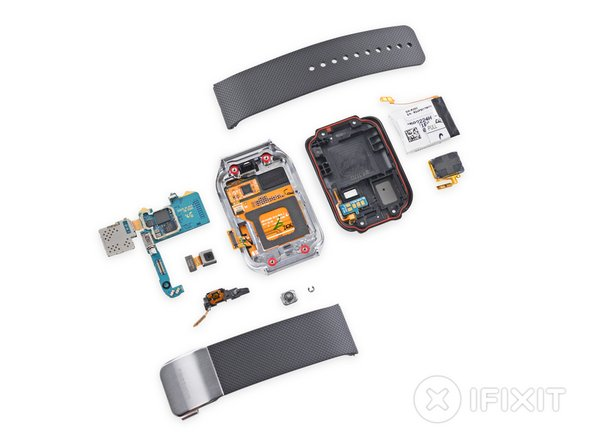
\includegraphics[width=\textwidth]{images/gear2-ifixit.jpg}

      \begin{center}
        {\tiny (from \url{https://www.ifixit.com/})}
      \end{center}
    \end{column}

  \end{columns}

\end{frame}

\begin{frame}{Many types of computers \insertcontinuationtext}
  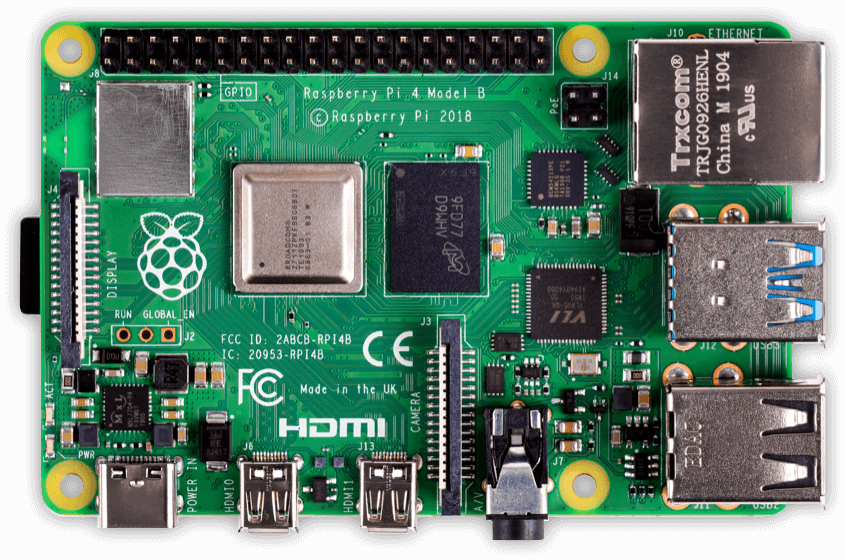
\includegraphics[width=\textwidth]{images/rpi-compressed.png}

  {\tiny (from \url{https://www.raspberrypi.org/})}
\end{frame}

\begin{frame}{Many types of computers \insertcontinuationtext}
  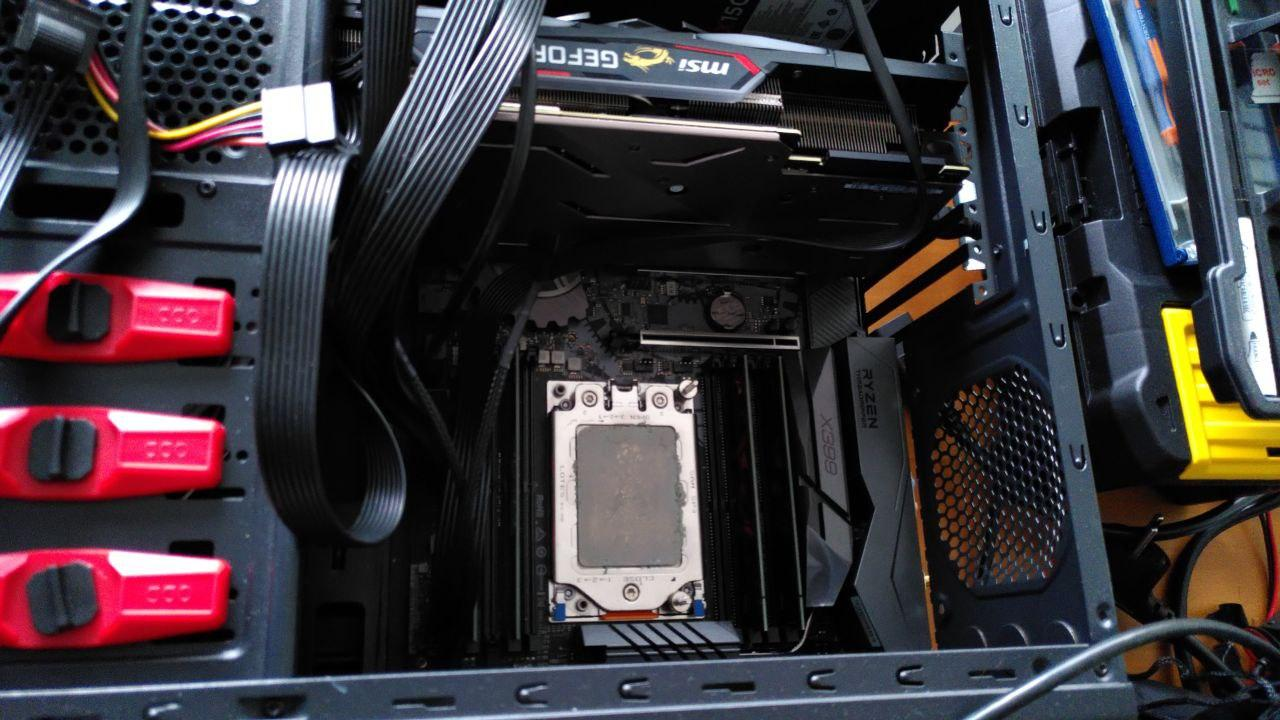
\includegraphics[width=\textwidth]{images/desktop.jpg}
\end{frame}

\begin{frame}{Many types of computers \insertcontinuationtext}
  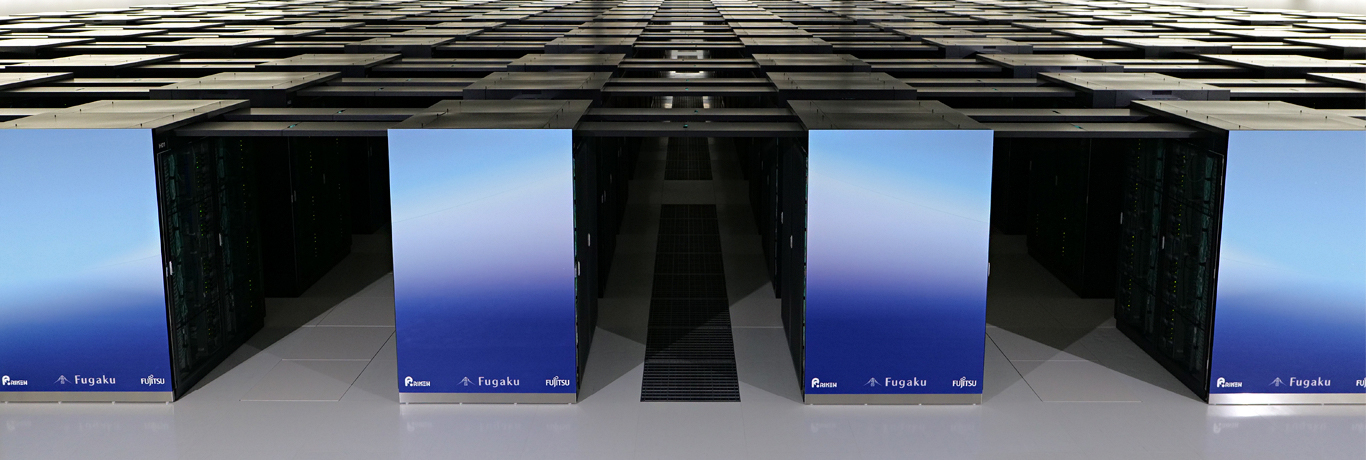
\includegraphics[width=\textwidth]{images/fugaku.jpg}

  {\tiny (from \url{https://www.riken.jp/en/})}
\end{frame}

\begin{frame}[label=current]{The Von Neumann architecture}

  \begin{center}

    \vskip -.8cm

    \begin{tikzpicture}[every text node part/.style={align=center}]
      \uncover<3->{
        \node[rectangle,draw,thick,minimum height=4cm,minimum width=2.1cm,fill=yellow,"Memory"] (memory) {
          data \\ + \\ instructions
        };
        \node[above=20pt of memory,inner sep=0pt,outer sep=0pt] (ram) {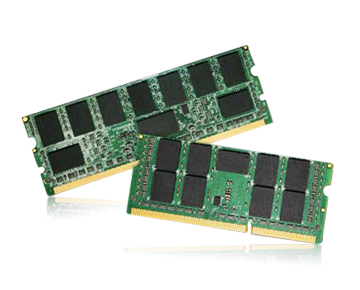
\includegraphics[height=1cm]{images/ram.jpg}};
      }
      \uncover<2->{
        \node[rectangle,black,draw,thick,minimum height=4cm,minimum width=2.5cm,fill=red!80!black,right=of memory,"CPU"] (cpu) {};
        \node[rectangle,black,draw,thick,text width=2cm,minimum
        height=1cm,fill=white,below=10pt of cpu.north,inner sep=0pt,outer sep=0pt] (alu) {\scriptsize
          Arithmetic-Logic Unit};
        \node[rectangle,black,draw,thick,minimum width=2cm,fill=white,above=of cpu.south] (control) {\scriptsize Control};
        \path (alu) -- (control) node[midway,rectangle,black,draw,thick,minimum width=2cm,fill=white] (registers) {\scriptsize Registers};
        \node[above=20pt of cpu,inner sep=0pt,outer sep=0pt] (intel) {
\includegraphics[height=1cm]{images/cpu.jpg}};
      }
      \uncover<3->{\draw[<->,thick] (memory) -- (cpu);}
      \uncover<4->{
        \node[tape,draw,thick,minimum height=1.5cm,minimum width=2cm,fill=green,right=of cpu.north east,yshift=-1cm] (input) {Input};
        \node[tape,draw,thick,minimum height=1.5cm,minimum width=2cm,fill=green,right=of cpu.south east,yshift=1cm] (output) {Output};
        \draw[<-,thick] (cpu) -- (input);
        \draw[->,thick] (cpu) -- (output);
        \node[above=of input,outer sep=0pt,inner sep=0pt] (keyboard) {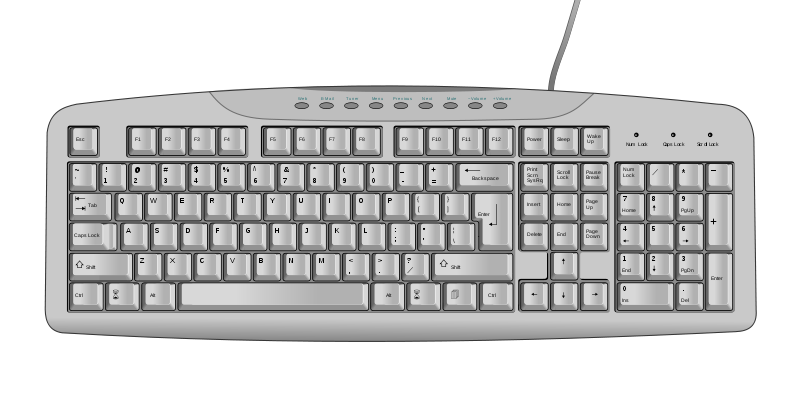
\includegraphics[height=1cm]{images/keyboard.png}};
        \node[right=0pt of keyboard] (mouse) {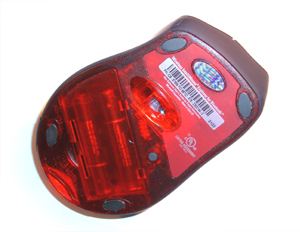
\includegraphics[height=1cm]{images/mouse.jpg}};
        \node[below right=0pt and 0pt of mouse,xshift=-.5cm] (monitor) {
\includegraphics[height=1cm]{images/monitor.png}};
        \node[below=0pt of monitor] (harddisk) {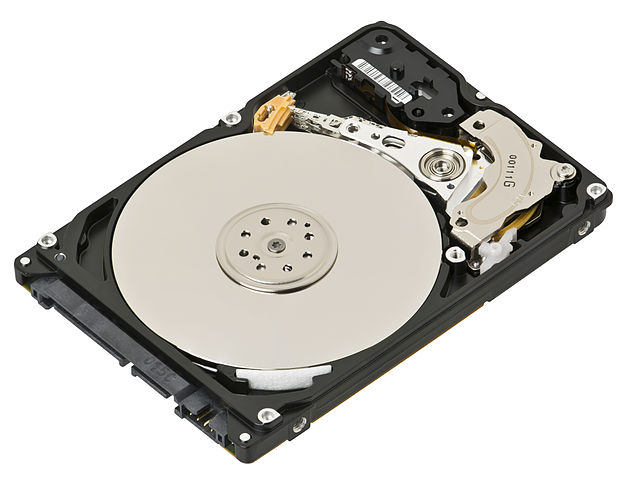
\includegraphics[height=1cm]{images/harddisk.jpg}};
        \node[below=0pt of harddisk] (usb-stick) {
\includegraphics[height=1cm]{images/usb-stick.png}};
        \node[below=0pt of usb-stick] (router) {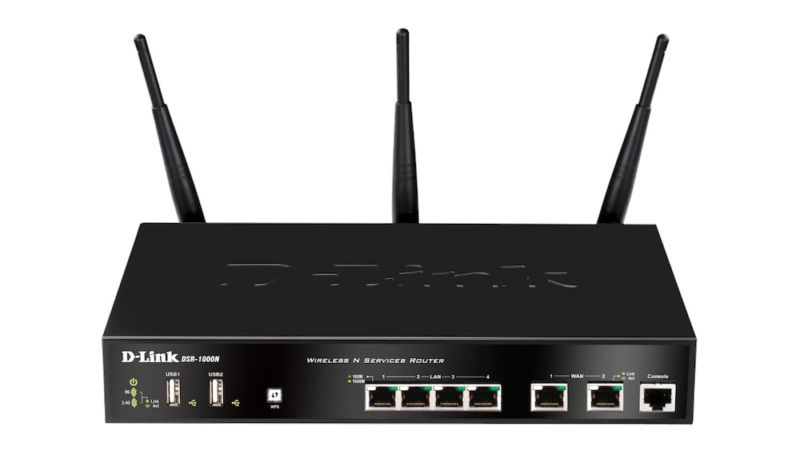
\includegraphics[height=1cm]{images/router.jpg}};
        \node[below left=0pt and 0pt of router] (gpu) {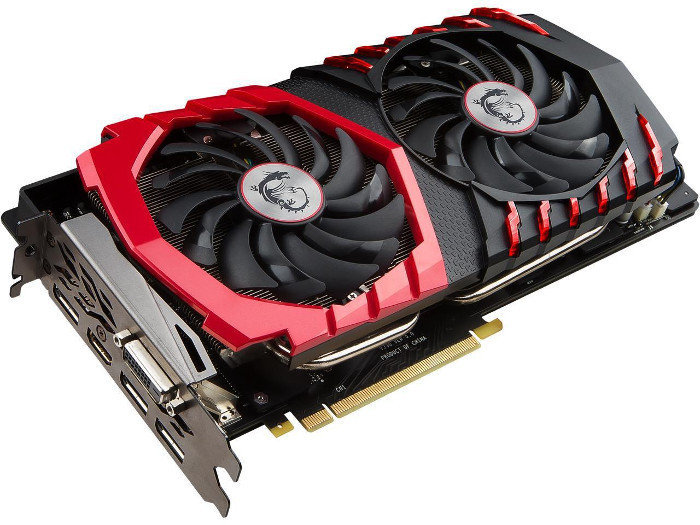
\includegraphics[height=1cm]{images/gpu.jpg}};
        \node[left=0pt of gpu] (sensor) {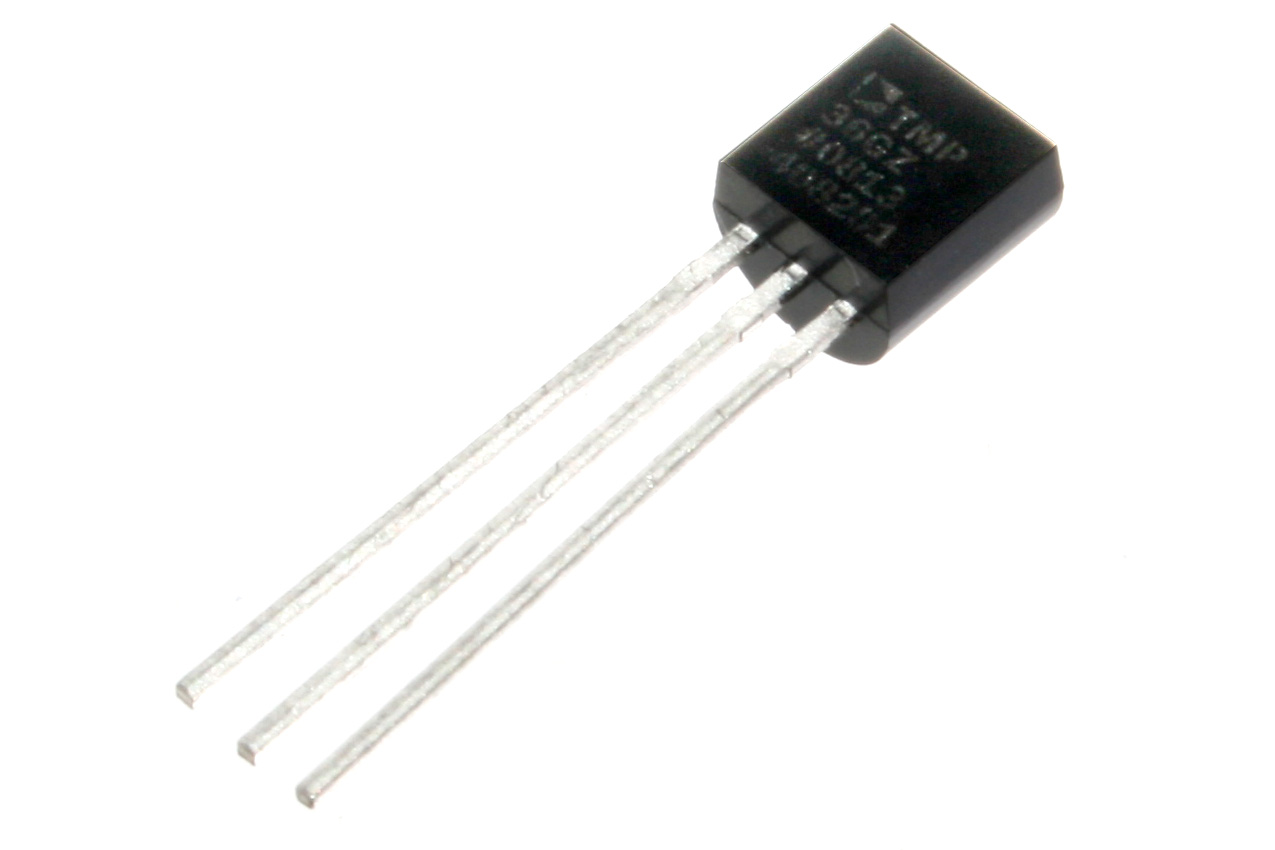
\includegraphics[height=1cm]{images/sensor.jpg}};
      }
    \end{tikzpicture}
  \end{center}

\end{frame}

\begin{frame}{The Von Neumann architecture \insertcontinuationtext}

  \begin{itemize}[<+->]
  \item Imagine memory as a looooong tape divided into locations whose content
    you can read and write
  \item Each memory location is identified by an index
    \begin{itemize}[<.->]
    \item e.g. location at position 8'363'944
    \end{itemize}
  \item Programs and the data they manage stay both in memory, typically in
    different regions
  \item The CPU fetches instructions from memory into its registers and executes
    them
  \item Typical instructions:
    \begin{itemize}[<.->]
    \item read data from memory into registers
    \item write data from registers to memory
    \item manipulate data in registers
    \end{itemize}
  \end{itemize}
\end{frame}

\begin{frame}[fragile]{Also data are binary}

  \begin{semiverbatim}
{\color{gray}00101001110110011000011111010111001011100111101100
11101000101001101011100111111100011101001000011010
00000110001101000011111010010001000101110000010010
00111011010111101101111110110011011111101100101101
10010010110011001101110011000011001011000001010010
11110100101111010001111001011000000000001111110100
1001110110001101101001\tikzref{ins}0110000101101111000000001101
00010001111001101000111100100110110110001101100100
01000110010111100011100010100101011011000110010001
10100011111101101000000000111101000001000100101101
11101100011010111001111110010101010110010010000100
00000010010011111010111011011101110011101100000111
00001001111011000000110000100110000101000100111011}\end{semiverbatim}

\uncover<2->{
  \tikz[overlay] \node[draw,thick,rounded corners,red,minimum width=65mm,minimum
  height=5mm] (data) at (ins) {};
  \tikz[overlay] \node[red] (description) at ([yshift=-35mm]data.south)
  {\only<3>{integer number 1667850607?}\only<4>{floating-point
      number $4.30511 \times 10^{21}$?}\only<5>{character string "ciao"?}};
}

\end{frame}

\begin{frame}[fragile]{A minimal C++ program}

  \begin{itemize}
  \item This program does nothing, successfully (details will be explained)
    \begin{codeblock}
int main() \{\}\end{codeblock}

  \item<2-> Let's write these 13 characters (including spaces) in a
    \alert{source file}, which we call \code{minimal.cpp}

  \begin{shellblock}<3->{
\$\tikzref{prompt} \uncover<4->{code minimal.cpp\tikzref{command}} \uncover<5->{\inserthitenter\tikzref{hitnewline}}
\uncover<6->{\$ cat minimal.cpp \inserthitenter
int main() \{\}
\$}}\end{shellblock}

\uncover<3>{\tikz[remember picture,overlay] \draw[<-,white] ([xshift=1ex] prompt) -- +(1,0) node[white,right] {\scriptsize this is the shell prompt};}
\uncover<4>{\tikz[remember picture,overlay] \draw[<-,white] ([xshift=1ex] command) -- +(1,0) node[white,right] {\scriptsize this is the command you write};}
\uncover<5>{\tikz[remember picture,overlay] \draw[<-,white] ([xshift=1ex] hitnewline) -- +(1,0) node[white,right] {\scriptsize you hit the ``Enter'' key on the keyboard};}

  \item<7> Before \alert{executing} the program we need to translate it into
    the language of the computer
  
  \end{itemize}

\end{frame}

\begin{frame}[fragile]{A minimal C++ program \insertcontinuationtext}

  \begin{itemize}

  \item In C++ the translation into a binary format is the job of the compiler,
    which produces an \alert{executable} file

\begin{center}
    \begin{tikzpicture}[every text node part/.style={align=center}]
      \node[tape,tape bend height=.3cm,draw,thick,inner sep=2pt,minimum height=2cm,minimum width=3cm] (source) {Source file \\ {\scriptsize(\code{minimal.cpp})}};
      \node[tape,tape bend height=.3cm,black,draw,thick, inner sep=2pt,minimum height=2cm,minimum width=3cm,right=3cm of source] (exe) {Executable binary file \\ {\scriptsize(\code{a.out})}};
      \draw[->] (source) -- (exe) node[above,align=center,midway] {Compilation \\ {\scriptsize(\code{g++})}};
    \end{tikzpicture}
  \end{center}

  \begin{shellblock}<2->{
\$ g++ minimal.cpp
\$ \uncover<3->{ls
a.out  minimal.cpp
\$ }\uncover<4->{./a.out\tikzref{program}
\$ }\uncover<5->{g++ minimal.cpp -o minimal
\$ ls
a.out  minimal  minimal.cpp
\$ }\uncover<6->{./minimal
\$ }}\end{shellblock}

  \uncover<4>{\tikz[remember picture,overlay] \draw[<-,white] ([xshift=1ex] program) -- +(1,0) node[white,right] {\scriptsize this command executes the program};}

  \item<7-> The \code{-o} option passed to the \code{g++} command allows to give
    another name to the final executable
  \end{itemize}

\end{frame}

\begin{frame}[fragile]{Spaces}

  \begin{itemize}
  \item Spaces are (almost) irrelevant
  \end{itemize}

  \begin{columns}[T]
  \begin{column}{.3\textwidth}<2->
    \begin{codeblock}
int main()\{\}

\end{codeblock}
  \end{column}

  \begin{column}{.3\textwidth}<3->
    \begin{codeblock}
int
main(  ) \{
   \}\end{codeblock}
  \end{column}

  \begin{column}{.3\textwidth}<4->
    \begin{codeblock}
int\tikzref{n1}main()\{ \}

    \end{codeblock}
  \end{column}

  \uncover<5->{
\begin{tikzpicture}[remember picture,overlay]
  \node[circle,radius=7pt,draw,red,line width=1pt,opacity=.7] at (n1) (n2){};
  \node[above=of n2,draw=red,line width=1pt,opacity=.7,rounded corners] {space needed here} edge[->,line width=1pt,red,opacity=.7] (n2);
\end{tikzpicture}
  }

\end{columns}

\begin{itemize}[<6->]
\item Tools exist to consistently format source code to improve readability
  \begin{itemize}
  \item They are customizable
  \item You are required to use them
  \end{itemize}
\end{itemize}

\begin{columns}[T]
  \begin{column}{.4\textwidth}
    \begin{shellblock}<7->{
\$ clang-format minimal.cpp
int main()
\{
\}
\$}\end{shellblock}
  \end{column}

  \begin{column}{.6\textwidth}
  \begin{codeblock}<8->{
# .clang-format file
\ldots
AllowShortFunctionsOnASingleLine: false
BraceWrapping:
  AfterFunction:   true
  \ldots}\end{codeblock}
  \end{column}
\end{columns}

\end{frame}

\begin{frame}[fragile]{Syntax check}

  \begin{itemize}
  \item The compiler can translate a program into a binary executable only if the
    code is syntactically correct

  \begin{codeblock}<2->{
intmain() \{\}}\end{codeblock}

  \begin{shellblock}<2->{
\$ g++ minimal.cpp
minimal.cpp:1:9: error: ISO C++ forbids declaration of \upquote{intmain} with \ldots
    1 | intmain() \{\}
      |         ^
\$}\end{shellblock}

  \item<3-> Error messages are usually precise about the cause of the error, but
    not always
  \item<3-> Learn to interpret error messages
  \end{itemize}

\end{frame}

\begin{frame}[fragile]{Comments}

  \begin{itemize}

  \item Code can contain comments

    \begin{codeblock}<2->{
int main() \alert{//} comment until the end of the line
\{
\}}\end{codeblock}

    \begin{codeblock}<3->{
int main()
\{
  \alert{/*} possibly multi-line comment
     that goes until the final marker
     and cannot nest \alert{*/}
\}}\end{codeblock}

  \item<4-> Comments are ignored by the compiler and are equivalent to spaces
  \item<4-> Comment are for humans
  \end{itemize}

\end{frame}

\begin{frame}[fragile]{Basic notions of Input and Output}

  \begin{itemize}
  \item The input and output system allows a program to interact with the
    external world
  \item One mechanism offered by C++ to do input and output is the \textit{I/O
      streams} interface, which allows the creation and the manipulation of
    \textit{stream} entities
    \begin{itemize}
    \item Values are extracted from an input stream
    \item Values are inserted into an output stream
    \end{itemize}
  \item Input and output streams connected to the terminal are automatically
    available to a program
    \begin{itemize}
    \item \code{std::cin}, \code{std::cout} (and \code{std::cerr} for errors)
    \end{itemize}
  \item To extract and insert values, use the stream \textit{operators}
    \code{>>} and \code{<<}, respectively
  \end{itemize}

\end{frame}

\begin{frame}[fragile]{Hello}

  A less minimal C++ program (details will be explained)

  \begin{codeblock}
\alert<2>{#include <iostream>}\uncover<2->{ // import I/O utilities}
\alert<2>{#include <string>}\uncover<2->{ // import string utilities}

int \alert<3>{main}()\uncover<3->{ // start the program from here}
\{
\alert<4>{  std::cout <{}< "What\textquotesingle{}s your name? ";}\uncover<4->{ // print a message on the terminal}
\alert<5>{  std::string name;}\uncover<5->{ // some space is needed in memory for a string}
\alert<6>{  std::cin >{}> name;}\uncover<6->{ // read a string from the terminal into that space}
\alert<7>{  std::cout <{}< "Hello, " <{}< name <{}< \bslashn{};}\uncover<7->{ // print a multi-part message}
\}\end{codeblock}

\begin{shellblock}<8->{
\uncover<8->{\$ g++ hello.cpp -o hello \inserthitenter
\$ }\uncover<9->{./hello \inserthitenter
What\textquotesingle{}s your name? }\uncover<10->{Francesco \inserthitenter
Hello, Francesco
\$ }}\end{shellblock}

\end{frame}

\begin{frame}{Objects}

  \begin{itemize}[<+->]
  \item The constructs in a C++ program create, destroy, refer to, access,
    and manipulate \alert<.>{objects}
  \item An object is a region of storage (i.e. memory)
    \begin{itemize}[<+->]
    \item has a \alert<.>{storage duration}/\alert<.>{lifetime}
    \item has a \alert<.>{type}
    \item can have a \alert<.>{name}
    \end{itemize}
  \end{itemize}

\end{frame}

\begin{frame}{Types}

  \begin{itemize}[<+->]
  \item A type gives meaning to a piece of storage
    \begin{itemize}
    \item What's the meaning of a piece of storage that contains $01100011011010010110000101101111$?
    \item Read as a sequence of alphabetic characters, it's the letters
      \textit{c}, \textit{i}, \textit{a}, \textit{o}
    \item Read as an integer number, it's $1667850607$
    \item Read as a floating-point number, it's about $4.30511 \times 10^{21}$
    \end{itemize}
  \item A type identifies a set of values and the operations that can be applied
    to those values
    \begin{itemize}
    \item C++ is a \alert{strongly typed} language (mostly)
    \end{itemize}
  \item The compiler checks that program instructions are compatible with the type system
    \begin{itemize}
    \item C++ is a \alert{statically typed} language (mostly)
    \end{itemize}
  \item A type is also associated with a machine representation for
    the values belonging to the type
  \item C++ defines a few fundamental types and provides mechanisms to build
    compound types on top of them
  \end{itemize}

\end{frame}

\begin{frame}{Fundamental types}
  \begin{itemize}
    \item arithmetic types
      \begin{itemize}
        \item integral types
          \begin{itemize}
          \item signed integer types: \code{short int}, \alert<3->{\code{int}},
            \code{long int}, \code{long long int}
          \item unsigned integer types: \code{unsigned short int},
            \code{unsigned int}, \code{unsigned long int}, \code{unsigned long
              long int}
          \item character types: \alert<3->{\code{char}}, \code{signed char},
            \code{unsigned char}, \ldots
          \item boolean types: \alert<3->{\code{bool}}
          \end{itemize}
        \item floating-point types: \code{float}, \alert<3->{\code{double}}, \code{long double}
      \end{itemize}
    \item \code{std::nullptr_t}
    \item \code{void}
  \end{itemize}

  \pause

  In general, size and machine representation are not defined by the
  standard

\end{frame}

\begin{frame}[fragile]{\code{int}}

  \begin{columns}
    \begin{column}{.8\textwidth}
      Type representing a signed integer number

      \begin{itemize}
      \item<2-> Set of values: subset of $\mathbb{Z}$
      \item<3-> Operations: addition, subtraction, multiplication, division,
        remainder, comparisons, \ldots
      \item<4-> Representation: 2's complement
      \item<5-> With N bits, values are in the range $[-2^{N-1}, 2^{N-1}-1]$
      \item<6-> Intended to have the natural size suggested by the architecture.
        Typical size is 32 bits (4 bytes)
        \begin{itemize}
        \item $[-2$ $147$ $483$ $648, +2$ $147$ $483$ $647]$
        \end{itemize}
      \end{itemize}
    \end{column}
    \hfill
    \begin{column}{.2\textwidth}
      \uncover<4->{\begin{tabular}{ r | r }
        7 & \alert{0}111 \\
        6 & \alert{0}110 \\
        5 & \alert{0}101 \\
        4 & \alert{0}100 \\
        3 & \alert{0}011 \\
        2 & \alert{0}010 \\
        1 & \alert{0}001 \\
        0 & \alert{0}000 \\
        -1 & \alert{1}111 \\
        -2 & \alert{1}110 \\
        -3 & \alert{1}101 \\
        -4 & \alert{1}100 \\
        -5 & \alert{1}011 \\
        -6 & \alert{1}010 \\
        -7 & \alert{1}001 \\
        -8 & \alert{1}000
      \end{tabular}}
    \end{column}
  \end{columns}

\end{frame}

\begin{frame}[fragile]{Variables}

  \begin{itemize}
  \item A variable is a \alert{name} for an \textit{object}
  \item A name is an \textit{identifier}: a sequence of letters (including
    \code{_}) and digits, starting with a letter
    \begin{itemize}
    \item Avoid \code{_} at the beginning
    \item Choose meaningful names
    \end{itemize}
  \end{itemize}

  \begin{codeblock}<2->{
\uncover<2->{int i;            // declaration}\uncover<3->{; the value is undefined}
\uncover<4->{i = 4321;         // assignment of a constant}
\uncover<5->{int j = 1234;     // declaration and initialization}
\uncover<6->{i = j;            // assignment of j\textquotesingle{}s value to i}}\end{codeblock}

  \begin{tikzpicture}[
      mem/.style={
        node font=\ttfamily\scriptsize,
        minimum height=.5cm,
      },
      location/.style={
        mem,
        draw=black!50,
        minimum width=1.2cm,
        fill=green!20!white,
      },
      every node/.style={
        mem,
      },
      anchor=south west,
      node distance=0,
    ]
    \clip (0.1,-1) rectangle (\textwidth-0.1cm,1.5);
    %% \visible<3->{\draw[step=.5cm,gray,thin,dashed] (0, .1cm) grid (\textwidth,0.4cm);}
    \visible<2->{\node at (0,0) [mem,draw=black!50,minimum width=\textwidth,
        "Memory" above] {};}
      \visible<2->{\node at (2,0) [location, "i" below] {
          \alt<-2>{}{\alt<3>{?}{\alt<4-5>{4321}{1234}}}};}
        \visible<5->{\node at (7,0) [location, "j" below] {1234};}
  \end{tikzpicture}

  \uncover<7->{NB At the end \code{i} and \code{j} have the same value but remain
  \alert{distinct} objects}

\end{frame}

\begin{frame}{Keywords}

  The following identifiers are reserved
  \vskip .5cm

  {
    \setbeamerfont{localfont}{size=\scriptsize,family=\tt}
    \usebeamerfont{localfont}

    \begin{tabular}{l l l l l l}
      alignas  & const        & for       & private          & throw    \\
      alignof  & constexpr    & friend    & protected        & true     \\
      and      & const_cast   & goto      & public           & try      \\
      and_eq   & continue     & if        & register         & typedef  \\
      asm      & decltype     & inline    & reinterpret_cast & typeid   \\
      auto     & default      & int       & return           & typename \\
      bitand   & delete       & long      & short            & union    \\
      bitor    & do           & mutable   & signed           & unsigned \\
      bool     & double       & namespace & sizeof           & using    \\
      break    & dynamic_cast & new       & static           & virtual  \\
      case     & else         & noexcept  & static_assert    & void     \\
      catch    & enum         & not       & static_cast      & volatile \\
      char     & explicit     & not_eq    & struct           & xor      \\
      char16_t & export       & nullptr   & switch           & xor_eq   \\
      char32_t & extern       & operator  & template         & wchar_t  \\
      class    & false        & or        & this             & while    \\
      compl    & float        & or_eq     & thread_local
    \end{tabular}
  }
\end{frame}

\begin{frame}{Literals}

  A literal is a constant \textbf{value} of a certain \textbf{type} included in
  the source code

  \pause

  \begin{itemize}
  \item integer
  \item floating point
  \item character
  \item string
  \item boolean
  \item \code{nullptr}
  \end{itemize}

\end{frame}

\begin{frame}{Integer literals}

  \begin{description}[<+->]
  \item[decimal] non-\code{0} decimal digit followed by zero or more digits
    \begin{itemize}[<.->]
    \item \code{1 -98 123456789 -1\textquotesingle{}234\textquotesingle{}567\textquotesingle{}890}
    \end{itemize}
  \item[binary] \code{0b} or \code{0B} followed by binary digits
    \begin{itemize}[<.->]
    \item \code{0b1101111010101101 0B111\textquotesingle{}0101\textquotesingle{}1011\textquotesingle{}1100\textquotesingle{}1101\textquotesingle{}0001\textquotesingle{}0101}
    \end{itemize}
  \item[exadecimal] \code{0x} or \code{0X} followed by hexadecimal digits
    \begin{itemize}[<.->]
    \item \code{-0xdead 0xDEad123f 0XdeAD\textquotesingle{}123F}
    \end{itemize}
  \item[octal] \code{0} followed by octal digits
    \begin{itemize}[<.->]
    \item \code{01 -077 07\textquotesingle{}654\textquotesingle{}321}
    \item N.B. A \code{0} in front of a number is meaningful!
    \end{itemize}
  \end{description}

  \uncover<+->{Integer literals are of type \code{int}}

\end{frame}

\begin{frame}[fragile]{\code{std::string}}

  \begin{itemize}[<+->]

  \item A \textit{compound} (\textit{user-defined}) type to represent a
    string of characters
  \item Provided by the C++ Standard Library
  \item Many operations available
  \item An \code{std::string} can be initialized with a string literal, a
    sequence of escaped or non-escaped characters between double quotes
    \begin{itemize}[<.->]
    \item \code{"hello" "hello\bslashn{}world" "hello
        \bslash{"}world\bslash{"}"}
    \item \code{\bslash{}n} means ``newline''
    \end{itemize}
  \item The type of a string literal is \textbf{not} \code{std::string}
  \end{itemize}

  \begin{codeblock}<+->{
std::string corso = "Programmazione per la Fisica";
\uncover<+->{corso = corso \tikzref{strplusref}+ "\bslash{n}Anno Accademico 2021/2022";}}\end{codeblock}

\uncover<+->{
  \begin{tikzpicture}[remember picture,overlay]
    \node[draw=red,line width=1pt,opacity=.7,rounded corners, minimum
    width=1.5ex] at ([xshift=.5ex]strplusref) (strplusbox) {};
    \node[below=of strplusbox,draw=red,line width=1pt,opacity=.7,rounded
    corners] {concatenate} edge[->,line width=1pt,red,opacity=.7] (strplusbox)
    {};
  \end{tikzpicture}
}

\end{frame}

\begin{frame}[fragile]{Expressions}

  \begin{itemize}
  \item An expression is a sequence of operators and their operands
    that specifies a computation
  \item Literals and variables are typical operands, but there are others

  \begin{codeblock}<2->{
\uncover<2->{1 + 2}
\uncover<3->{\alert<8->{i = 1 + 2}       // assignment}
\uncover<4->{i == j          // equality comparison}
\uncover<5->{sqrt(x) > 1.42}
\uncover<6->{\alert<8->{std::cout <{}< "hello, " <{}< name <{}< \upquote{\bslash{}n}}}}\end{codeblock}

\item<7-> The evaluation of an expression typically produces a result
\item<8-> Some expressions have \textit{side-effects}
  \begin{itemize}
  \item They modify the state of the program, i.e. the state of memory, or the
    external world
  \end{itemize}

\end{itemize}

\end{frame}

\begin{frame}[fragile]{Operators}

  \begin{columns}[t]

    \column{0.12\textwidth}
    {\scriptsize Arithmetic}
    \begin{codeblock}
+a
-a
a + b
a - b
a * b
a / b
a % b
~a
a & b
a | b
a ^ b
a {<}< b
a {>}> b\end{codeblock}

    \column{0.12\textwidth}
    \centering{\scriptsize Logical}
    \begin{codeblock}
!a
a && b
a || b\end{codeblock}

    \column{0.13\textwidth}
    \centering{\scriptsize Comparison}
    \begin{codeblock}
a == b
a != b
a {<} b
a {>} b
a {<}= b
a >= b\end{codeblock}

    \column{0.13\textwidth}
    \centering{\scriptsize Increment}
    \begin{codeblock}
++a
{-}-a
a++
a{-}-\end{codeblock}

    \column{0.14\textwidth}
    \centering{\scriptsize Assignments}
    \begin{codeblock}
a = b
a += b
a -= b
a *= b
a /= b
a %= b
a &= b
a |= b
a ^= b
a <{}<= b
a >{}>= b\end{codeblock}

    \column{0.09\textwidth}
    \centering{\scriptsize Access}
    \begin{codeblock}
a[b]
*a
&a
a->b
a.b\end{codeblock}

    \column{0.09\textwidth}
    \centering{\scriptsize Other}
    \begin{codeblock}
a(\ddd)
a, b
? :\end{codeblock}

  \end{columns}

  \vskip .5cm % bleah!

  Plus: casts, allocation and deallocation, static introspection, \ldots

  \begin{itemize}[<+->]
  \item Rules exist for associativity, commutativity and precedence
    \begin{itemize}
    \item When in doubt use parentheses
    \end{itemize}
  \item Many operators can be \alert{overloaded} for user-defined
    types
    \begin{itemize}[<.->]
    \item e.g. \code{+} to concatenate strings
    \end{itemize}
  \end{itemize}

\end{frame}

\begin{frame}{Algorithm}

  A finite sequence of precisely defined steps to solve a problem

\end{frame}

\begin{frame}<1-2>[fragile,label=firstexample]{Sum of two numbers}

  A program that reads two numbers from input and writes their sum to output

  \begin{columns}[T]
    \begin{column}{.5\textwidth}
      \centering
  \uncover<2->{
    \begin{tikzpicture}
      [auto,
      startstop/.style = {rectangle, rounded corners=5pt, draw=black, thick, node font=\scriptsize,
        text width=4em, align=flush center},
      inout/.style     = {trapezium, trapezium left angle=60,trapezium right angle=120, thick, draw=green, fill=green!20,
        text width=4em, align=flush center, node font=\scriptsize},
      block/.style     = {rectangle, draw=blue, thick, fill=blue!20,align=center, rounded corners=2pt,
        text width=4em, align=flush center, node font=\scriptsize},
      decision/.style  = {diamond, aspect=1.5, draw=red, thick, fill=red!20, text width=4em, align=flush center, inner sep=1pt, node font=\scriptsize},
      line/.style      = {draw, thick, -latex, shorten >=2pt}]
      \matrix [column sep=5mm,row sep=4mm]
      {
        % row 1
        \node [startstop] (start) {start}; \\
        % row 2
        \node [inout] (in) {read a, b}; \\
        % row 3
        \node [block,text width=7em] (result) {result $\leftarrow$ a + b}; \\
        % row 4
        \node [inout] (out) {write result}; \\
        % row 5
        \node [startstop] (stop) {stop}; \\
      };
      \begin{scope}[every path/.style=line]
        \path (start)  -- (in);
        \path (in)     -- (result);
        \path (result) -- (out);
        \path (out)    -- (stop);
      \end{scope}
    \end{tikzpicture}
  }
    \end{column}
    \begin{column}{.5\textwidth}
      \begin{codeblock}<3->{
#include <iostream>

int main()
\{
  \uncover<4->{\alert<4>{int a;
  int b;
  std::cin >{}> a >{}> b;}}
  \uncover<5->{\alert<5>{int result = a + b;}}
  \uncover<6->{\alert<6>{std::cout <{}< result <{}< \bslashn;}}
\}}\end{codeblock}

    \end{column}
  \end{columns}

  \uncover<7->{}
\end{frame}

\begin{frame}{Statement}
  Statements are units of code that are executed in sequence

  \begin{itemize}
  \item expression statement
  \item compound statement or block
  \item declaration statement
  \item selection statement
  \item iteration statement
  \item jump statement
  \item \ldots
  \end{itemize}

\end{frame}

\againframe<3->{firstexample}

\begin{frame}[fragile]{Expression statement}

  \begin{itemize}[<+->]
  \item An expression followed by a semicolon (\code{;})
  \item The value of the expression (if any) is discarded
  \item The expression can have side effects
  \end{itemize}

  \begin{codeblock}
\uncover<1->{b + 2;}
\uncover<3->{a = b + 2;
std::cin >{}> a >{}> b;}
\uncover<4->{; // empty statement}\end{codeblock}

\end{frame}

\begin{frame}[fragile]{Compound statement (or block)}

  A sequence of zero or more statements enclosed between braces
  (\code{\{\}})

  \begin{codeblock}
\{
   found = true;
   ++i;
   int n = 3;
   std::cout <{}< n;
\}\end{codeblock}

  \begin{codeblock}
\{ found = true; ++i; \ddd \} // all on one line\end{codeblock}

\end{frame}

\begin{frame}{Declaration statement}

  \begin{itemize}[<+->]
  \item A declaration statement introduces one or more new identifiers into a
    \Cpp{} program, possibly initializing them
    \begin{itemize}
    \item typically variables, but not only
    \end{itemize}

  \item A declaration of a \textbf{variable} in a \textbf{block} makes the
    variable of \alert{automatic storage duration}, unless otherwise specified
    \begin{itemize}
    \item the corresponding object is automatically created each time the
      declaration is executed
    \item<.-> the corresponding object is automatically destroyed each time the
      execution reaches the end of the block
    \end{itemize}

  \item A declaration should introduce only one identifier

  \item A variable should be declared only in the moment it's actually needed

  \item A variable should be initialized at the point of declaration, if there
    is a meaningful initial value

  \end{itemize}

\end{frame}

\begin{frame}[fragile]{The smallest of two numbers}

  A program that reads two numbers from input and writes the smallest to output

  \begin{columns}[T]
    \begin{column}{.5\textwidth}
  \uncover<2->{
    \begin{tikzpicture}
      [auto,
      startstop/.style = {rectangle, rounded corners=5pt, draw=black, thick, node font=\scriptsize,
        text width=3em, align=flush center},
      inout/.style     = {trapezium, trapezium left angle=60,trapezium right angle=120, thick, draw=green, fill=green!20,
        text width=4em, align=flush center, node font=\scriptsize},
      block/.style     = {rectangle, draw=blue, thick, fill=blue!20,align=center, rounded corners=2pt,
        text width=5em, align=flush center, node font=\scriptsize},
      decision/.style  = {diamond, aspect=1.5, draw=red, thick, fill=red!20, text width=4em, align=flush center, inner sep=1pt, node font=\scriptsize},
      line/.style      = {draw, thick, -latex, shorten >=2pt}]
      \matrix [column sep=0mm,row sep=4mm,ampersand replacement=\&]
      {
        % row
        \& \node [startstop] (start) {start}; \\
        % row
        \& \node [inout] (in) {read a, b}; \\
        % row
        \& \node [decision] (less) {a < b}; \\[-4mm]
        % row
        \node [block] (a) {result $\leftarrow$ a}; \&
        \& \node [block] (b) {result $\leftarrow$ b}; \\
        % row
        \& \coordinate (join); \\
        % row
        \& \node [inout] (out) {write result}; \\
        % row
        \& \node [startstop] (stop) {stop}; \\
      };
      \begin{scope}[every path/.style=line]
        \path (start)  -- (in);
        \path (in)     -- (less);
        \path (less)   -| node [near start,above] {\scriptsize{yes}} (a);
        \path (less)   -| node [near start,above] {\scriptsize{no}} (b);
        \path[-,shorten >=0pt] (a)   |- (join);
        \path[-,shorten >=0pt] (b)   |- (join);
        \path (join) -- (out);
        \path (out)    -- (stop);
      \end{scope}
    \end{tikzpicture}
  }
    \end{column}
    \begin{column}{.5\textwidth}
      \begin{codeblock}<3->{
#include <iostream>

int main()
\{
  \uncover<4->{\alert<4>{int a;
  int b;
  std::cin >{}> a >{}> b;}}
  \uncover<9->{\alert<9>{int result;}}
  \uncover<5->{\alert<5>{if (a < b) \{}
    \uncover<6->{\alert<6>{\only<-8>{int }result = a;}}
  \alert<5>{\} else \{}
    \uncover<6->{\alert<6>{\only<-8>{int }result = b;}}
  \alert<5>{\}}}
  \uncover<7->{\alert<7>{std::cout <{}< result <{}< \bslashn;}}\uncover<8>{\alert<8>{ // error}}
\}}\end{codeblock}

    \end{column}
  \end{columns}

  \uncover<10->{}

\end{frame}

\begin{frame}[fragile]{\code{if then else}}

  \begin{itemize}
  \item<1-> Selection statement to choose one of two flows of control depending on a
    boolean condition
  \item<2-> Two (basic) forms:
    \begin{itemize}
    \item<3-> \code{if (} \textit{condition-expr} \code{)} \textit{statement} \code{else} \textit{statement}
    \item<4-> \code{if (} \textit{condition-expr} \code{)} \textit{statement}
    \end{itemize}

  \begin{columns}[t]

    \begin{column}{.45\textwidth}

      \begin{codeblock}<3->{
\alert{if} (a < b) \{
  result = a;   // "true" branch
\} \alert{else} \{
  result = b;   // "false" branch
\}}\end{codeblock}

    \end{column}

    \begin{column}{.45\textwidth}
      \begin{codeblock}<4->{
int i = \ddd;
\alert{if} (i < 0) \{
  i = -i;   // "true" branch
\}}\end{codeblock}

    \end{column}

  \end{columns}

  \item<5-> \textit{condition-expr} can be any expression whose result is of type
    (convertible to) \code{bool}, i.e. either true or false

  \item<6-> \textit{statement} can be a block, possibly including multiple
    statements
    \begin{itemize}
    \item In fact, the statement should always be a block
    \end{itemize}
  \end{itemize}

\end{frame}

\begin{frame}[fragile]{\code{bool}}

  Type representing a boolean value
  \begin{itemize}
  \item Set of values: ${false, true}$
  \item Operations: conjunction (\textit{and}), disjunction (\textit{or}),
    negation (\textit{not}), \ldots
  \item Size: typically $1$ byte
  \item Representation: like the \code{int}s \code{0} and \code{1}
  \item Literals: \code{false} and \code{true}

    \begin{codeblock}<2->{
\uncover<2->{bool b = true;}
\uncover<3->{b \tikzref{aref}= i =\tikzref{eref}= j;}
\uncover<6->{bool b2 = i !\tikzref{neref}= 1234;}
\uncover<7->{bool b3 = b2 \alert<7>{\&\&} i < j;    // and
bool b4 = i < j \alert<7>{||} i < k; // or
bool b5 = \alert<7>{!}\alert<8>{(}i == j\alert<8>{)};      // not}}\end{codeblock}

  \item<8-> Note the use of parenthesis in \code{!(i == j)} to have the right
    precedence of application of operators
  \end{itemize}

\uncover<4->{
  \begin{tikzpicture}[remember picture,overlay]
    \uncover<4-5>{
      \node[draw=red,line width=1pt,opacity=.7,rounded corners, minimum width=1.5ex] at ([xshift=.5ex]aref) (abox){};
      \node[below=of abox,draw=red,line width=1pt,opacity=.7,rounded corners] {assignment} edge[->,line width=1pt,red,opacity=.7] (abox);
    }
    \uncover<5>{
      \node[draw=red,line width=1pt,opacity=.7,rounded corners,minimum width=3ex] at (eref) (ebox){};
      \node[below right=of ebox.south east,draw=red,line width=1pt,opacity=.7,rounded corners] {equality} edge[->,line width=1pt,red,opacity=.7] (ebox);
    }
    \uncover<6>{
      \node[draw=red,line width=1pt,opacity=.7,rounded corners,minimum width=3ex] at (neref) (nebox){};
      \node[below=of nebox,draw=red,line width=1pt,opacity=.7,rounded corners] {inequality} edge[->,line width=1pt,red,opacity=.7] (nebox);
    }
  \end{tikzpicture}
}

\end{frame}

\begin{frame}{Logical operations}

  \begin{description}[<+->]

  \item[and] Both operands are true
    \vskip .5em
    {\scriptsize\begin{tabular}{ c c | c }
      op1 & op2 & op1 \textbf{\&\&} op2 \\
      \hline
      \code{false} & \code{false} & \code{false} \\
      \code{false} & \code{true} & \code{false} \\
      \code{true} & \code{false} & \code{false} \\
      \code{true} & \code{true} & \code{true} \\
    \end{tabular}}
    \vskip .5em

    \code{op2} is evaluated only if \code{op1} is \code{true}

  \item[or] At least one operand is true
    \vskip .5em

    {\scriptsize\begin{tabular}{ c c | c }
      op1 & op2 & op1 \textbf{||} op2 \\
      \hline
      \code{false} & \code{false} & \code{false} \\
      \code{false} & \code{true} & \code{true} \\
      \code{true} & \code{false} & \code{true} \\
      \code{true} & \code{true} & \code{true} \\
    \end{tabular}}
    \vskip .5em

    \code{op2} is evaluated only if \code{op1} is \code{false}

  \item[not] Operand's negation (or logical complement)
    \vskip .5em

    {\scriptsize\begin{tabular}{ c | c }
      op & \textbf{!}op \\
      \hline
      \code{false} & \code{true} \\
      \code{true}  & \code{false} \\
    \end{tabular}}
    \vskip .5em

  \end{description}

\end{frame}

\begin{frame}{Scope}

  The scope of a name appearing in a program is the, possibly
  discontiguous, portion of source code where that name is valid

  \begin{itemize}
  \item block scope
  \item function scope
  \item class scope
  \item namespace scope (including the global one)
  \item \ldots
  \end{itemize}

\end{frame}

\begin{frame}[fragile]{Block scope}

  \begin{itemize}[<+->]
  \item The scope of a name declared in a block starts at the point of
    declaration and ends at the \code{\}}

    \begin{codeblock}
\{
  \ddd
  int num;         // scope of num begins here
  std::cin >{}> num; // ok
\}                  // scope of num ends here
std::cout <{}< num;  // error\end{codeblock}

  \item<2-> The scope of a variable should be as small as possible
    \begin{itemize}
    \item Declare a variable only when it's needed
    \item If possible/meaningful, initialize it
    \end{itemize}
  \end{itemize}

\end{frame}

\begin{frame}[fragile]{Example: is a number even?}

  A program that reads a number from input and tells if it's even

  \begin{columns}[T]
    \begin{column}{.6\textwidth}
  \uncover<2->{
    \begin{tikzpicture}
      [auto,
      startstop/.style = {rectangle, rounded corners=5pt, draw=black, thick, node font=\scriptsize,
        text width=3em, align=flush center},
      inout/.style     = {trapezium, trapezium left angle=60,trapezium right angle=120, thick, draw=green, fill=green!20,
        text width=4em, align=flush center, node font=\scriptsize},
      block/.style     = {rectangle, draw=blue, thick, fill=blue!20,align=center, rounded corners=2pt,
        text width=5em, align=flush center, node font=\scriptsize},
      decision/.style  = {diamond, aspect=1.5, draw=red, thick, fill=red!20, text width=4em, align=flush center, inner sep=1pt, node font=\scriptsize},
      line/.style      = {draw, thick, -latex, shorten >=2pt}]
      \matrix [column sep=0mm,row sep=4mm,ampersand replacement=\&]
      {
        % row
        \& \node [startstop] (start) {start}; \\
        % row
        \& \node [inout] (in) {read num}; \\
        % row
        \& \node [block,text width=7em] (mod) {r $\leftarrow$ num \textit{mod} 2}; \\
        % row
        \& \node [decision] (iszero) {r == 0}; \\[-4mm]
        % row
        \node [block,text width=6em] (even) {result $\leftarrow$ true}; \&
        \& \node [block,text width=6em] (odd) {result $\leftarrow$ false}; \\
        % row
        \& \coordinate (join); \\
        % row
        \& \node [inout,text width=6em] (out) {write result}; \\
        % row
        \& \node [startstop] (stop) {stop}; \\
      };
      \begin{scope}[every path/.style=line]
        \path (start)  -- (in);
        \path (in)     -- (mod);
        \path (mod)    -- (iszero);
        \path (iszero) -| node [near start,above] {\scriptsize{yes}} (even);
        \path (iszero) -| node [near start,above] {\scriptsize{no}} (odd);
        \path[-,shorten >=0pt] (even) |- (join);
        \path[-,shorten >=0pt] (odd)  |- (join);
        \path (join) -- (out);
        \path (out)    -- (stop);
      \end{scope}
    \end{tikzpicture}
  }
    \end{column}

    \begin{column}{.4\textwidth}
      \begin{codeblock}<3->{
#include <iostream>

int main()
\{
\uncover<4->{\alert<4>{  int num;
  std::cin >{}> num;}}
\uncover<5->{\alert<5>{  int r = num \% 2;}}
\only<7-10>{\alert<7>{  bool result;}}\only<11->{  bool result \alert<11>{= r == 0};}
\only<6-10>{\alert<6>{  if (r == 0) \{}}
\only<7-10>{\alert<7>{    result = true;}}
\only<6-10>{\alert<6>{  \} else \{}}
\only<7-10>{\alert<7>{    result = false;}}
\only<6-10>{\alert<6>{  \}}}
\only<9>{  // print 0/1}\only<10>{  // print false/true}
\only<8-9>{\alert<8>{  std::cout <{}< result <{}< \bslashn;}}\only<10->{  std::cout <{}< \alert<10>{std::boolalpha}
      <{}< result <{}< \bslashn;}
\}}\end{codeblock}
    \end{column}

  \end{columns}

\end{frame}

\begin{frame}{Exercise: the smallest of three numbers}

  Write a program that reads three numbers from standard input and writes the
  smallest one to standard output

\end{frame}

\begin{frame}[fragile]{Integer square root}

  Write a program that computes the integer square root of a non-negative
  integer number, i.e. the largest integer number whose square is not greater
  than the given number

  \begin{columns}[T]
    \begin{column}{.5\textwidth}
      \uncover<2->{\begin{tikzpicture}
          [auto,
          startstop/.style = {rectangle, rounded corners=5pt, draw=black, thick, node font=\scriptsize,
            text width=3em, align=flush center},
          inout/.style     = {trapezium, trapezium left angle=60,trapezium right angle=120, thick, draw=green, fill=green!20,
            text width=4em, align=flush center, node font=\scriptsize},
          block/.style     = {rectangle, draw=blue, thick, fill=blue!20,align=center, rounded corners=2pt,
            text width=5em, align=flush center, node font=\scriptsize},
          decision/.style  = {diamond, aspect=1.5, draw=red, thick, fill=red!20, text width=4em, align=flush center, inner sep=1pt, node font=\scriptsize},
          line/.style      = {draw, thick, -Classical TikZ Rightarrow, shorten >=1pt}]
          \matrix [column sep=4mm,row sep=3mm,ampersand replacement=\&]
          {
            % row
            \& \node [startstop] (start) {start}; \\
            % row
            \& \node [inout] (in) {read $n$}; \\
            % row
            \& \node [block] (initi) {$i \gets 1$}; \\[-1mm]
            % row
            \& \coordinate (beforecond1); \\
            % row
            \node [block] (inc) {$i \gets i + 1$}; \& \node [decision] (cond1) {$i \times i < n$}; \\
            % row
            \node [block] (dec) {$i \gets i - 1$};
            \& \node [decision] (cond2) {$i \times i > n$}; \\[-1mm]
            % row
            \& \coordinate (aftercond2); \\
            % row
            \& \node [inout] (out) {write $i$}; \\
            % row
            \& \node [startstop] (stop) {stop}; \\
          };
          \begin{scope}[every path/.style=line]
            \path (start)  -- (in);
            \path (in)     -- (initi);
            \path (initi)  -- (cond1);
            \path (cond1)  -- node {\scriptsize{no}} (cond2);
            \path (cond1)  -- node {\scriptsize{yes}} (inc);
            \path (inc)    |- (beforecond1);
            \path (cond2)  -- node [near start] {\scriptsize{no}} (out);
            \path (cond2)  -- node {\scriptsize{yes}} (dec);
            \path (dec)    |- (aftercond2);
            \path (out)    -- (stop);
          \end{scope}
        \end{tikzpicture}}

    \end{column}

    \begin{column}{.5\textwidth}
      \begin{codeblock}<3->{
#include <iostream>

int main()
\{
  int n;
  std::cin >> n;
  int i = 1;
  while (i * i < n) \{
    ++i;   // equivalent to i = i + 1
  \}
  if (i * i > n) \{
    --i;   // equivalent to i = i - 1
  \}
  std::cout << i << \bslashn;
\}}\end{codeblock}
    \end{column}

  \end{columns}

\end{frame}

\begin{frame}[fragile]{\code{while} loop}

  \begin{center}
    \code{while (} \textit{condition-expr} \code{)} \textit{statement}
  \end{center}

  \pause

  \begin{itemize}[<+->]
  \item Execute repeatedly \textit{statement} until \textit{condition-expr}
    becomes false
  \item \textit{condition-expr} is evaluated at the beginning of each iteration
    \begin{itemize}
    \item If \textit{condition-expr} is already \code{false} at the beginning,
      \textit{statement} is never executed
    \end{itemize}
  \item \textit{statement} can be any statement, including of course a block
  \item \textit{statement} should modify something so that the evaluation of
    \textit{condition-expr} may change
    \begin{itemize}[<.->]
    \item Otherwise the loop may never terminate
    \end{itemize}
  \end{itemize}

\end{frame}

\begin{frame}[fragile]{Sum of the first N numbers}
  Write a program that reads a non-negative integer number N from standard
  input, computes the sum of the first N numbers and writes the result to
  standard output

  \begin{columns}[T]

    \begin{column}{.5\textwidth}
      \begin{codeblock}<2->{
#include <iostream>

int main()
\{
  int n;
  std::cin >{}> n;
  int sum = 0;
  \alert<3->{int i = 1;}
  while (\alert<3->{i <= n}) \{
    sum += i;   // sum = sum + i
    \alert<3->{++i};
  \}
  std::cout <{}< sum <{}< \bslashn;
\}}\end{codeblock}

    \end{column}

    \begin{column}{.5\textwidth}
      \begin{codeblock}<4->{
#include <iostream>

int main()
\{
  int n;
  std::cin >{}> n;
  int sum = 0;

  \textbf<4>{for} (\alert<4>{int i = 1}; \alert<4>{i <= n}; \alert<4>{++i}) \{
    sum += i;

  \}
  std::cout <{}< sum <{}< \bslashn;
\}}\end{codeblock}
    \end{column}

  \end{columns}
\end{frame}

\begin{frame}[fragile]{\code{for} loop}

  \code{for (} \textit{init-statement} \opt{\textit{condition-expr}} \code{;}
  \opt{\textit{expression}} \code{)} \textit{statement}

  \pause

  \begin{itemize}[<+->]
  \item Execute \textit{init-statement}, which may be a single \code{;}
    \begin{itemize}
    \item If \textit{init-statement} contains declarations (e.g. the \code{i}
      variable in the previous example), the scope of the declared names is
      the loop
    \end{itemize}
  \item Execute repeatedly \textit{statement} until \textit{condition-expr} becomes false
  \item \textit{condition-expr} is evaluated at the beginning of each iteration
    \begin{itemize}
    \item If \textit{condition-expr} is already false at the beginning,
      \textit{statement} is never executed
    \item But \textit{init-statement} is always executed
    \end{itemize}
  \end{itemize}

\end{frame}

\begin{frame}[fragile]{\code{for} loop \insertcontinuationtext}

  \code{for (} \textit{init-statement} \opt{\textit{condition-expr}} \code{;}
  \opt{\textit{expression}} \code{)} \textit{statement}

  \pause

  \begin{itemize}[<+->]
  \item \textit{expression} is evaluated at the end of each iteration
  \item \textit{statement} and/or \textit{expression} should modify something so
    that the evaluation of \textit{condition-expr} may change
    \begin{itemize}[<.->]
    \item Otherwise the loop may never terminate
    \end{itemize}
  \item A \code{for} loop can always be transformed into a \code{while} loop and
    viceversa
    \begin{itemize}
    \item Prefer a \code{for} loop when there is an obvious loop variable
    \end{itemize}
  \end{itemize}
\end{frame}

\begin{frame}[fragile]{Integer square root with a \code{for} loop}

  Write a program that computes the integer square root of a non-negative
  integer number, i.e. the largest integer number whose square is not greater
  than the given number

  \begin{columns}[T]
    \begin{column}{.35\textwidth}
      \begin{codeblock}
#include <iostream>

int main()
\{
  int n;
  std::cin >{}> n;
  int i = 1;
  while (i * i < n) \{
    ++i;
  \}
  if (i * i > n) \{
    --i;
  \}
  std::cout << i << \bslashn;
\}\end{codeblock}
    \end{column}

    \begin{column}{.65\textwidth}
      \begin{codeblock}<2->{
#include <iostream>

int main()
\{
  int n;
  std::cin >{}> n;
  \uncover<4->{int i = 1;}
  for (\alt<-3>{int i = 1}{ }; i * i < n; ++i) \alt<-5>{\{}{\alert<6>{;}}
    \only<-4>{;}
  \only<-5>{\}}
  if (\alert<3>{i} * \alert<3>{i} > n) \{\uncover<3>{ // \alert{error: undeclared variable}}
    --\alert<3>{i};
  \}
  std::cout << i << \bslashn;
\}}\end{codeblock}
    \end{column}

  \end{columns}

  \uncover<7>{}

\end{frame}

\begin{frame}{Exercise: the smallest of N numbers}

  Write a program that reads an arbitrary sequence of numbers from standard
  input and writes the smallest one to standard output

  Hint 1: press Ctrl-D to tell the program there is nothing more to read from
  standard input

  Hint 2: the expression \code{std::cin.good()} tells if it's still possible to
  read something from \code{std::cin}
\end{frame}

\begin{frame}[fragile]{\code{double}}

  Type representing a floating-point number

  \begin{itemize}
  \item<2-> Set of values: subset of $\mathbb{R}$
  \item<3-> Operations: addition, subtraction, multiplication, division, comparisons, \ldots
  \item<4-> Representation: \href{https://en.wikipedia.org/wiki/IEEE_754}{IEEE 754}
  \item<5-> 64 bits, smallest values $\approx\pm10^{-308}$, largest values $\approx\pm10^{308}$
  \item<6-> Precision is about 16 decimal digits
  \item<6-> Literals in the form \opt{\textit{sign}} \textit{significand} \opt{\textit{exponent}}
    \begin{itemize}
    \item \code{42.0 1. -1.5 12.34e3 -.34E-3 -1234e-2}
    \item \code{\ddd{}e\textit{n}}/\code{\ddd{}E\textit{n}} means $\times 10^{n}$
    \end{itemize}
  \end{itemize}
\end{frame}

\begin{frame}[fragile]{\code{float}}

  Type representing a floating-point number

  \begin{itemize}
  \item<2-> Set of values: subset of $\mathbb{R}$
  \item<3-> Operations: addition, subtraction, multiplication, division, comparisons, \ldots
  \item<4-> Representation: \href{https://en.wikipedia.org/wiki/IEEE_754}{IEEE 754}
  \item<5-> 32 bits, smallest values $\approx\pm10^{-38}$, largest values $\approx\pm10^{38}$
  \item<6-> Precision is about 7 decimal digits
  \item<6-> Literals in the form \opt{\textit{sign}} \textit{significand} \opt{\textit{exponent}} \code{F}
    \begin{itemize}
    \item \code{42.0f 1.F -1.5f 12.34e3F -.34E-3f -1234e-2F}
    \item Same as double but with an \code{f} or \code{F} suffix
    \end{itemize}
  \end{itemize}
\end{frame}

\begin{frame}[fragile]{Handle floating-point numbers with care}

  \begin{itemize}
  \item<1-> Floating-point numbers are \textbf{not} real numbers
    \begin{itemize}
    \item Finite representation $\implies$ there is a previous and a next
    \end{itemize}
  \item<2-> When managing floating-point numbers one should take into account
    rounding errors and inexact representations
    \begin{codeblock}<3->{
float x = 1\textquotesingle000\textquotesingle000\textquotesingle000;
\uncover<4->{std::cout << std::setprecision(10)
  << x - 32 << \upquote{ } << x << \upquote{ } << x + 32}\uncover<5->{ // 1000000000 1000000000 1000000000}
\uncover<6->{  << x + 32 - x << \upquote{ } << x - x + 32;}\uncover<7->{    // 0 32}}\end{codeblock}
  \item<8-> Floating-point math in general is not associative
  \item<9-> When comparing floating-point numbers avoid the use of equality
 \end{itemize}

\end{frame}

\begin{frame}[fragile]{Standard mathematical functions}

  The \href{https://en.cppreference.com/w/cpp/header/cmath}{\code{cmath}} header
  includes many ready-to-use mathematical functions
  \begin{itemize}
  \item Exponential
  \item Power
  \item Trigonometric
  \item Interpolation
  \item Hyperbolic
  \item Floating-point manipulation, classification and comparison
  \item \ldots
  \end{itemize}

  \begin{codeblock}<2->{
#include <cmath>
\ddd
double x = \ddd;
std::sqrt(x);
std::pow(x, .5);
std::sin(x);
std::log(x);
std::abs(x);}\end{codeblock}
\end{frame}

\begin{frame}[fragile]{Type conversions}

    \begin{itemize}
    \item A value of type \code{T1} may be converted \textbf{implicitly} to a
      value of type \code{T2} in order to match the expected type in a certain
      situation
      \begin{codeblock}<2->{
1 + 2.3}\end{codeblock}
      \begin{itemize}[<3->]
      \item between numbers and bool
      \item between signed and unsigned numbers
      \item between numbers of different size
      \item between integral and floating-point numbers
      \item \ldots
      \end{itemize}

    \item<4-> Conversions sometimes are surprising
    \item<5-> Conversions can be explicit using \code{static_cast}
      \begin{codeblock}<.->{
1 + static_cast<int>(2.3)}\end{codeblock}
    \item<6-> Mechanims exist to define implicit and explicit conversions
      involving user-defined types

    \end{itemize}

\end{frame}

\begin{frame}[fragile]{\code{const}-safety}

  \begin{itemize}
  \item Data qualified as \code{const} is logically immutable
  \item Data that is meant to be immutable should be \code{const}
  \end{itemize}

  \begin{codeblock}<2->{
int \alert{const} x = 1\textquotesingle000\textquotesingle000\textquotesingle000; // or const int
\uncover<3->{std::cout << x + 32;    // ok, read-only}
\uncover<4->{x += 32;                // error, trying to modify}
\uncover<5->{int const y;            // error, not initialized and not modifiable later}
}\end{codeblock}

\begin{codeblock}<6->{
std::string \alert{const} message = "Hello";
\uncover<7->{std::cout << message + " Francesco";      // ok, read-only}
\uncover<8->{message += " Francesco";                  // error, trying to modify}
\uncover<9->{std::string const empty_message;          // ok! empty string}}\end{codeblock}

  \begin{itemize}[<10->]
  \item Primitive types (e.g. \code{int}) and user-defined types such as
    \code{std::string}) behave differently with respect to \textit{default
      initialization}, i.e. without an explicit initial value
    \begin{itemize}
    \item User-defined types can define what default initialization means
    \item For \code{std::string} it means ``empty string''
    \item More later
    \end{itemize}
  \end{itemize}

\end{frame}

\begin{frame}{Functions}

  \begin{itemize}[<+->]
  \item A function abstracts away a piece of code that performs a well-defined
    task behind a well-defined interface
  \item A function associates a block of statements with
    \begin{itemize}
    \item a name
    \item a list of zero or more parameters
    \end{itemize}
  \item A function may return a result
  \end{itemize}

  \begin{itemize}[<+->]
  \item Let's consider the code that computes the integer square root
    \begin{itemize}
    \item Let's give it a name $\rightarrow$ \code{isqrt}
    \item We pass \code{isqrt} a number $\rightarrow$ the list of parameters has
      only one item of type \code{int}
    \item \code{isqrt} computes a value that we want back $\rightarrow$ the
      function returns a value of type \code{int}
    \end{itemize}
  \end{itemize}

\end{frame}

\begin{frame}[fragile]{The \code{isqrt} function}

  \begin{columns}[T]
    \begin{column}{.5\textwidth}
      \begin{codeblock}
#include <iostream>

int main()
\{
  int n;
  std::cin >{}> n;
  int i = 1;
  while (i * i < n) \{
    ++i;
  \}
  if (i * i > n) \{
    --i;
  \}
  std::cout << i << \bslashn;
\}\end{codeblock}

      \vskip .5cm

      \uncover<2>{Names on the two sides of the call are independent}
    \end{column}

    \begin{column}{.5\textwidth}
      \begin{codeblock}
#include <iostream>

int isqrt(int \alert<2>{n})  \only<1>{// \alert{function definition}}
\{
  int i = 1;
  while (i * i < n) \{
    ++i;
  \}
  if (i * i > n) \{
    --i;
  \}
  return \alert<2>{i};      \only<1>{// \alert{return statement}}
\}

int main()
\{
  int \alt<1>{n}{\alert<2>{num}};
  std::cin >{}> \alt<1>{n}{\alert<2>{num}};
  int \alt<1>{i}{\alert<2>{result}} = isqrt(\alt<1>{n}{\alert<2>{num}});  \only<1>{// \alert{function call}}
  std::cout <{}< \alt<1>{i}{\alert<2>{result}} <{}< \bslashn;
\}\end{codeblock}
    \end{column}

  \end{columns}

\end{frame}

\begin{frame}{Functions \insertcontinuationtext}

  \begin{itemize}
  \item<1-> A function needs to be declared/defined before its use

    \textit{return-type} \textit{function-name} \code{(} \textit{parameter-list} \code{);}

    \textit{return-type} \textit{function-name} \code{(} \textit{parameter-list} \code{) \{ \ddd \}}

    \visible<2->{

      \code{int isqrt(int);}

      \code{int count_words(std::string s) \{ \ddd \}}

      \code{double pow(double base, double exponent);}

      \code{void print(std::string);}

      \code{int generate_random_number();}
    }

  \item<3-> Each parameter in the parameter list is of the form

    \textit{type \opt{name}}

    \textit{type} is mandatory, \textit{name} is optional

  \item<4-> Parameters are separated by commas

  \item<5-> The parameter list can be empty, i.e. \code{()}
  \item<6-> If the function returns nothing, the return type is \code{void}
  \end{itemize}

\end{frame}

\begin{frame}{Functions \insertcontinuationtext}

  \begin{itemize}

  \item<1-> A function has only one entry point, but it may have multiple exit
    points, i.e. there can be multiple \code{return} statements

    \begin{itemize}
    \item For a function returning a non-\code{void} type

      \code{return} \textit{expression}\code{;}

      The result of \textit{expression} must be convertible to the return type

    \item For a function returning \code{void}

      \code{return;}

      In this case the \code{return} is optional (at the end of the function)

    \end{itemize}

  \end{itemize}
\end{frame}

\begin{frame}{Functions \insertcontinuationtext}

  \begin{itemize}
  \item<1-> Calling/invoking a function is a type of expression of the form $F(E_1,
    E_2, \ldots, E_N)$
    \begin{itemize}
    \item $F$ is an expression that identifies a function, typically its name
    \item Each $E_i$ is an expression, whose value is used to initialize the
      corresponding parameter (i.e. in the same position) in the function
      declaration
    \end{itemize}

    \visible<2->{
      \code{int s = isqrt(24);}

      \code{std::cout << count_words("Hello, " + name);}

      \code{print(std::to_string(pow(isqrt(24), 2)));}
    }

  \item<3-> A function can call other functions
  \item<4-> A function should not be too long; if it is, try to break it into
    multiple parts, each implemented as a function
  \item<5-> A function can call itself, directly or indirectly
    \begin{itemize}
    \item This is called \textit{recursion}
    \item Often an elegant alternative to a loop
    \item Not easy to master, don't abuse
    \end{itemize}
  \end{itemize}

\end{frame}

\begin{frame}[fragile]{The \code{main} function}
  \begin{itemize}
  \item The \code{main} (special) function is the entry point of a program
  \item It can have two forms
    \begin{itemize}
    \item \code{int main() \{\ddd\}}
    \item \ldots (see later)
    \end{itemize}
  \item If there is no \code{return} statement, an implicit \code{return 0;} is assumed
    \begin{itemize}
    \item $0$ means success, different from $0$ means failure
    \item Or use \code{EXIT_SUCCESS} and \code{EXIT_FAILURE} from \code{<cstdlib>}
    \item The exit value is available to the shell via the \code{\$?} variable
    \end{itemize}
  \end{itemize}

  \begin{codeblock}<2->{
#include <cstdlib>

int main()
\{
  int n;
  std::cin >{}> n;
  if (std::cin.fail() || n < 0) \{
    std::cerr << "Invalid number\bslash{}n";
    return EXIT_FAILURE;
  \}
  \ddd
\}}\end{codeblock}

\end{frame}

\begin{frame}{Exercises}
  \begin{itemize}
  \item Write a function \code{pow} that takes two \code{int}s and computes and
    returns the value of the first (the base) raised to the power of the second
    (the exponent)
  \item Write a function \code{gcd} that takes two \code{int}s and computes the
    Gratest Common Denominator using the
    \href{https://en.wikipedia.org/wiki/Euclidean_algorithm}{Euclid's algorithm}
  \item Write a function \code{lcm} that takes two \code{int}s and computes the
    Least Common Multiple
  \item Write a function \code{is\_prime} that takes an \code{int} and tells if
    it's a prime number
  \item More on \href{https://edabit.com/}{edabit}, \href{https://leetcode.com/}{leetcode}, \ldots
  \end{itemize}

\end{frame}

\begin{frame}[fragile]{How do we know the code we write is correct?}

  \begin{itemize}[<+->]
  \item Correctness is the result of the application of multiple good practices
    to the software developmente process
  \item One of the most effective techniques is \textbf{testing}
    \begin{itemize}
    \item Execute the code with reasonable and unreasonable input and see if it
      behaves according to the expectations
    \item The purpose of testing is to (try to) \alert{break} the code
    \end{itemize}
  \item Here we focus on a form of testing called \textit{unit testing}, where
    the units (of code) under test are, for example, functions
  \item There are many tools/frameworks to do unit testing (Google Test, Catch,
    Doctest, Boost.Test, \ldots)
  \item Let's use \href{https://github.com/onqtam/doctest}{Doctest}
  \end{itemize}
\end{frame}

\begin{frame}[fragile]{How to use Doctest}

  \begin{itemize}
  \item On \href{https://godbolt.org/}{godbolt} it's available selecting it
    under ``Libraries''
  \item Otherwise download locally a single
    \href{https://raw.githubusercontent.com/onqtam/doctest/master/doctest/doctest.h}{\textit{header
        file}} into the directory containing your code, e.g. using \code{wget}
    or \code{curl}
  \item At the top of your C++ file add the lines
    \begin{codeblock}
#define DOCTEST\_CONFIG\_IMPLEMENT\_WITH\_MAIN
#include "doctest.h"\end{codeblock}
  \item Don't add \code{main} into your file
  \item After the code of the function(s) you have written, add lines like the
    following:
    \begin{codeblock}
TEST_CASE("Testing isqrt") \{
  CHECK(isqrt(0) == 0);
  CHECK(isqrt(9) == 3);
  CHECK(isqrt(10) == 3);
  CHECK(isqrt(-1) == 0);
  \ddd
\}\end{codeblock}

  \end{itemize}

\end{frame}

\begin{frame}{Memory layout of a process}

  \begin{itemize}
  \item A process is a running program
  \item When a program is started the operating system brings the contents of
    the corresponding file into memory according to well-defined conventions
  \end{itemize}

  \begin{columns}
    \begin{column}{.7\textwidth}
      \begin{itemize}
        \item[]
      \begin{itemize}
      \item Stack
        \begin{itemize}
        \item function local variables
        \item function call bookkeeping
        \end{itemize}
      \item Heap
        \begin{itemize}
        \item dynamic allocation
        \end{itemize}
      \item Global data
        \begin{itemize}
        \item literals and variables
        \item initialized and uninitialized (set to 0)
        \end{itemize}
      \item Program instructions
      \end{itemize}
    \end{itemize}
  \end{column}

    \begin{column}{.3\textwidth}
      \centering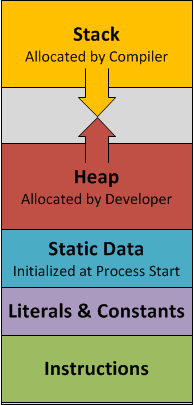
\includegraphics[height=.5\textheight]{images/process-memory-layout}
    \end{column}
  \end{columns}

\end{frame}

\begin{frame}[fragile]{Functions and the stack}

  \begin{columns}
    \begin{column}{.5\textwidth}
      \begin{codeblock}
\alert<4>{int isqrt(int n)
\{
  int i} \alert<6>{= 1};
  \alert<7>{while (i * i < n) \{
    ++i;
  \}
  if (i * i > n) \{
    --i;
  \}}
  \alert<8>{return i;}
\alert<4>{\}}

\alert<2>{int main()
\{
  int num};
  \alert<3>{std::cin >{}> num;}
  \alert<2>{int result} \alert<8>{=} \alert<4>{isqrt(}\alert<5>{num}\alert<4>{)};
  std::cout <{}< result <{}< \bslashn;
\alert<2>{\}}\end{codeblock}

    \end{column}

    \begin{column}{.4\textwidth}
      \begin{tikzpicture}[
        mem/.style={
          minimum width=2cm,
          inner sep=0pt,
          outer sep=0pt,
          draw=black
        },
        frame/.style={
          minimum width=2cm,
          inner sep=0pt,
          outer sep=0pt,
          draw=black,
          thick,
          fill=green!50!white
        },
        var/.style={
          node font=\ttfamily\scriptsize,
          minimum height=.5cm,
          minimum width=2cm,
          draw=black,
          fill=green!30!white,
          inner sep=0pt,
          outer sep=0pt
        },
        anchor=south west]
        \visible<1->{
          \node at (0,0) [
          mem,
          minimum height=7cm,
          label={90:Stack}] {};
        }
        \visible<2-9>{
          \node (main) at (0,4) [
            frame,
            minimum height=2cm,
            label={[yshift=.9cm]0:\scriptsize\tt main}
          ] {};
          \node (result) [
            var,
            above=3ex of main.south,
            label={180:\scriptsize\tt result}
          ] {\only<8->{2}};
          \node (num) [
            var,
            above=0pt of result,
            label={180:\scriptsize\tt num}
          ] {\only<3->{5}};
        }
        \visible<4-8>{
          \node (isqrt) [
            frame,
            below=0pt of main,
            minimum height=2cm,
            label={[yshift=.9cm]0:\scriptsize\tt isqrt}
          ] {};
          \node (i) [
            var,
            above=3ex of isqrt.south,
            label={180:\scriptsize\tt i}
          ] {\only<6>{1}\only<7->{2}};
          \node (n) [
            var,
            above=0pt of i,
            label={180:\scriptsize\tt n}
          ] {\only<5->{5}};
        }
        \visible<2-3,9>{
          \node (main rsp) at ([xshift=-2cm]main.south west) {\scriptsize\tt \%rsp};
          \draw[->] (main rsp) -- +(1.5cm,0);
        }
        \visible<4-8>{
          \node (isqrt rsp) at ([xshift=-2cm]isqrt.south west) {\scriptsize\tt \%rsp};
          \draw[->] (isqrt rsp) -- +(1.5cm,0);
        }
      \end{tikzpicture}
    \end{column}

  \end{columns}

  \uncover<10>{}

\end{frame}

\begin{frame}{Pass by-value, return by-value}

  Given a function

  % \tikzref doesn't work inside \code nor inside \texttt; to be investigated

  \begin{equation*}
    \code{R F(T$_1$ p}\tikzref{p1}\code{$_1$, \ddd, T$_n$ p}\tikzref{pn}\code{$_n$) \{ \ddd{} return E}\tikzref{er}\code{$_R$; \} }
  \end{equation*}

  and a function call

  \begin{equation*}
    \code{R r}\tikzref{r}\code{ = F(E}\tikzref{e1}\code{$_1$, \ddd, E}\tikzref{en}\code{$_n$);}
  \end{equation*}

  \begin{itemize}
  \item<2-> Each \code{p$_i$} is initialized as a \alert{copy} of the value of
    expression \code{E$_i$}
    \begin{itemize}
    \item If \code{E$_i$} is just a variable, changing \code{p$_i$} inside the
      function doesn't change the variable
    \end{itemize}
  \item<3-> \code{r} is initialized as a \alert{copy} of the value of expression
    \code{E$_R$}
  \end{itemize}

  \visible<2->{
    \tikz[remember picture, overlay] \draw[-Stealth,blue,line width=1pt] ([yshift=1ex] e1) -- ([yshift=-1ex]p1);
    \tikz[remember picture, overlay] \draw[-Stealth,blue,line width=1pt] ([yshift=1ex] en) -- ([yshift=-1ex]pn);
  }
  \visible<3->{
    \tikz[remember picture, overlay] \draw[-Stealth,brown,line width=1pt] ([yshift=-1ex] er) -- ([yshift=1ex]r);
  }

\end{frame}

\begin{frame}{Stack frame}

  \begin{itemize}[<+->]
  \item A piece of memory allocated and dedicated to the execution of a function
  \item It contains local variables (including function parameters), return
    address, saved registers, \ldots
  \item Managed in a Last-In, First-Out (LIFO) way
  \item The size of the stack frame is computed by the compiler
  \item There is a special register (the stack pointer register, \code{\%rsp})
    that indicates the frame of the currently running function
  \item At runtime the allocation/deallocation of a frame consists simply in
    subtracting/adding that frame size to the stack pointer register
  \end{itemize}
\end{frame}

